\documentclass{standalone}
\usepackage{tikz}
\usetikzlibrary{patterns}
\usetikzlibrary{positioning}
\usetikzlibrary{patterns, positioning}
\usetikzlibrary{shapes.misc}
\usepackage[outline]{contour}
\contourlength{1.5pt} 


\begin{document}
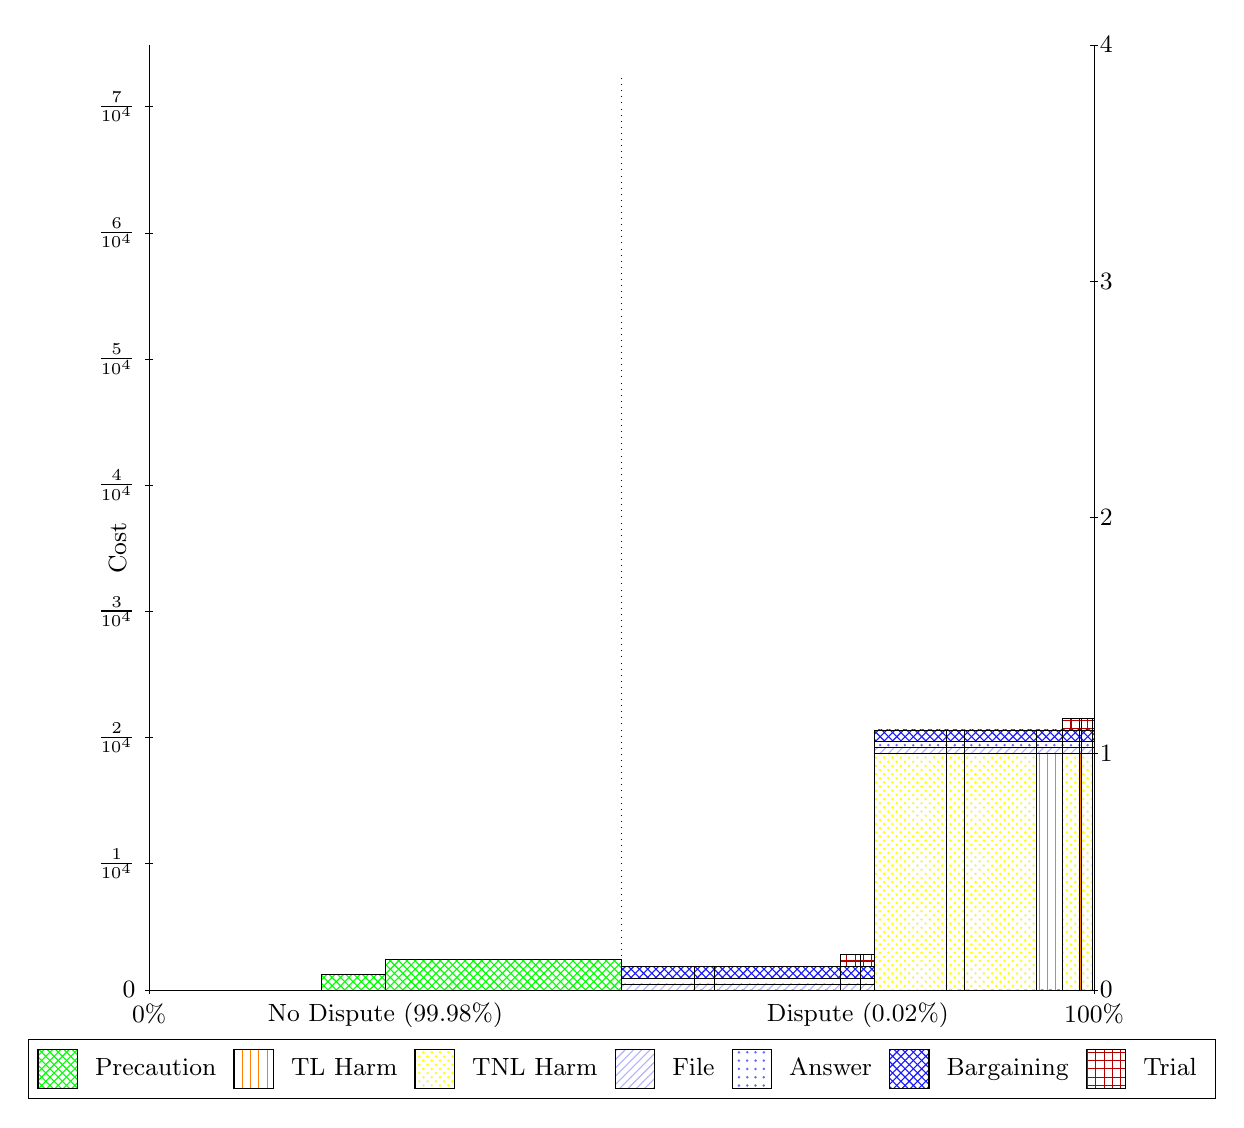
\begin{tikzpicture}
\draw[pattern=crosshatch, pattern color=green,draw=black,very thin] (3.6907,2.5) rectangle (4.5,2.6923);
\draw[pattern=crosshatch, pattern color=green,draw=black,very thin] (4.5,2.5) rectangle (7.5,2.8845);
\draw[pattern=north east lines, pattern color=blue!30,draw=black,very thin] (7.5,2.5) rectangle (8.4184,2.575);
\draw[pattern=dots,  pattern color=blue!60,draw=black,very thin] (7.5,2.575) rectangle (8.4184,2.65);
\draw[pattern=crosshatch,      pattern color=blue!90,draw=black,very thin] (7.5,2.65) rectangle (8.4184,2.8);
\draw[pattern=crosshatch, pattern color=green,draw=black,very thin] (8.4184,2.5) rectangle (8.673,2.5);
\draw[pattern=north east lines, pattern color=blue!30,draw=black,very thin] (8.4184,2.5) rectangle (8.673,2.575);
\draw[pattern=dots,  pattern color=blue!60,draw=black,very thin] (8.4184,2.575) rectangle (8.673,2.65);
\draw[pattern=crosshatch,      pattern color=blue!90,draw=black,very thin] (8.4184,2.65) rectangle (8.673,2.8);
\draw[pattern=crosshatch, pattern color=green,draw=black,very thin] (8.673,2.5) rectangle (10.275,2.5001);
\draw[pattern=north east lines, pattern color=blue!30,draw=black,very thin] (8.673,2.5001) rectangle (10.275,2.5751);
\draw[pattern=dots,  pattern color=blue!60,draw=black,very thin] (8.673,2.5751) rectangle (10.275,2.6501);
\draw[pattern=crosshatch,      pattern color=blue!90,draw=black,very thin] (8.673,2.6501) rectangle (10.275,2.8001);
\draw[pattern=north east lines, pattern color=blue!30,draw=black,very thin] (10.275,2.5) rectangle (10.527,2.575);
\draw[pattern=dots,  pattern color=blue!60,draw=black,very thin] (10.275,2.575) rectangle (10.527,2.65);
\draw[pattern=crosshatch,      pattern color=blue!90,draw=black,very thin] (10.275,2.65) rectangle (10.527,2.8);
\draw[pattern=grid,            pattern color=red!70!black,draw=black,very thin] (10.275,2.8) rectangle (10.527,2.95);
\draw[pattern=crosshatch, pattern color=green,draw=black,very thin] (10.527,2.5) rectangle (10.705,2.5);
\draw[pattern=north east lines, pattern color=blue!30,draw=black,very thin] (10.527,2.5) rectangle (10.705,2.575);
\draw[pattern=dots,  pattern color=blue!60,draw=black,very thin] (10.527,2.575) rectangle (10.705,2.65);
\draw[pattern=crosshatch,      pattern color=blue!90,draw=black,very thin] (10.527,2.65) rectangle (10.705,2.8);
\draw[pattern=grid,            pattern color=red!70!black,draw=black,very thin] (10.527,2.8) rectangle (10.705,2.95);
\draw[pattern=crosshatch dots, pattern color=yellow,draw=black,very thin] (10.705,2.5) rectangle (11.62,5.5);
\draw[pattern=north east lines, pattern color=blue!30,draw=black,very thin] (10.705,5.5) rectangle (11.62,5.575);
\draw[pattern=dots,  pattern color=blue!60,draw=black,very thin] (10.705,5.575) rectangle (11.62,5.65);
\draw[pattern=crosshatch,      pattern color=blue!90,draw=black,very thin] (10.705,5.65) rectangle (11.62,5.8);
\draw[pattern=vertical lines, pattern color=orange,draw=black,very thin] (11.62,2.5) rectangle (11.623,5.5);
\draw[pattern=north east lines, pattern color=blue!30,draw=black,very thin] (11.62,5.5) rectangle (11.623,5.575);
\draw[pattern=dots,  pattern color=blue!60,draw=black,very thin] (11.62,5.575) rectangle (11.623,5.65);
\draw[pattern=crosshatch,      pattern color=blue!90,draw=black,very thin] (11.62,5.65) rectangle (11.623,5.8);
\draw[pattern=crosshatch, pattern color=green,draw=black,very thin] (11.623,2.5) rectangle (11.854,2.5);
\draw[pattern=crosshatch dots, pattern color=yellow,draw=black,very thin] (11.623,2.5) rectangle (11.854,5.5);
\draw[pattern=north east lines, pattern color=blue!30,draw=black,very thin] (11.623,5.5) rectangle (11.854,5.575);
\draw[pattern=dots,  pattern color=blue!60,draw=black,very thin] (11.623,5.575) rectangle (11.854,5.65);
\draw[pattern=crosshatch,      pattern color=blue!90,draw=black,very thin] (11.623,5.65) rectangle (11.854,5.8);
\draw[pattern=crosshatch, pattern color=green,draw=black,very thin] (11.854,2.5) rectangle (11.855,2.5);
\draw[pattern=vertical lines, pattern color=orange,draw=black,very thin] (11.854,2.5) rectangle (11.855,5.5);
\draw[pattern=north east lines, pattern color=blue!30,draw=black,very thin] (11.854,5.5) rectangle (11.855,5.575);
\draw[pattern=dots,  pattern color=blue!60,draw=black,very thin] (11.854,5.575) rectangle (11.855,5.65);
\draw[pattern=crosshatch,      pattern color=blue!90,draw=black,very thin] (11.854,5.65) rectangle (11.855,5.8);
\draw[pattern=crosshatch, pattern color=green,draw=black,very thin] (11.855,2.5) rectangle (12.767,2.5001);
\draw[pattern=crosshatch dots, pattern color=yellow,draw=black,very thin] (11.855,2.5001) rectangle (12.767,5.5001);
\draw[pattern=north east lines, pattern color=blue!30,draw=black,very thin] (11.855,5.5001) rectangle (12.767,5.5751);
\draw[pattern=dots,  pattern color=blue!60,draw=black,very thin] (11.855,5.5751) rectangle (12.767,5.6501);
\draw[pattern=crosshatch,      pattern color=blue!90,draw=black,very thin] (11.855,5.6501) rectangle (12.767,5.8001);
\draw[pattern=crosshatch, pattern color=green,draw=black,very thin] (12.767,2.5) rectangle (13.09,2.5001);
\draw[pattern=vertical lines, pattern color=orange,draw=black,very thin] (12.767,2.5001) rectangle (13.09,5.5001);
\draw[pattern=north east lines, pattern color=blue!30,draw=black,very thin] (12.767,5.5001) rectangle (13.09,5.5751);
\draw[pattern=dots,  pattern color=blue!60,draw=black,very thin] (12.767,5.5751) rectangle (13.09,5.6501);
\draw[pattern=crosshatch,      pattern color=blue!90,draw=black,very thin] (12.767,5.6501) rectangle (13.09,5.8001);
\draw[pattern=crosshatch dots, pattern color=yellow,draw=black,very thin] (13.09,2.5) rectangle (13.313,5.5);
\draw[pattern=north east lines, pattern color=blue!30,draw=black,very thin] (13.09,5.5) rectangle (13.313,5.575);
\draw[pattern=dots,  pattern color=blue!60,draw=black,very thin] (13.09,5.575) rectangle (13.313,5.65);
\draw[pattern=crosshatch,      pattern color=blue!90,draw=black,very thin] (13.09,5.65) rectangle (13.313,5.8);
\draw[pattern=grid,            pattern color=red!70!black,draw=black,very thin] (13.09,5.8) rectangle (13.313,5.95);
\draw[pattern=vertical lines, pattern color=orange,draw=black,very thin] (13.313,2.5) rectangle (13.342,5.5);
\draw[pattern=north east lines, pattern color=blue!30,draw=black,very thin] (13.313,5.5) rectangle (13.342,5.575);
\draw[pattern=dots,  pattern color=blue!60,draw=black,very thin] (13.313,5.575) rectangle (13.342,5.65);
\draw[pattern=crosshatch,      pattern color=blue!90,draw=black,very thin] (13.313,5.65) rectangle (13.342,5.8);
\draw[pattern=grid,            pattern color=red!70!black,draw=black,very thin] (13.313,5.8) rectangle (13.342,5.95);
\draw[pattern=crosshatch, pattern color=green,draw=black,very thin] (13.342,2.5) rectangle (13.474,2.5);
\draw[pattern=crosshatch dots, pattern color=yellow,draw=black,very thin] (13.342,2.5) rectangle (13.474,5.5);
\draw[pattern=north east lines, pattern color=blue!30,draw=black,very thin] (13.342,5.5) rectangle (13.474,5.575);
\draw[pattern=dots,  pattern color=blue!60,draw=black,very thin] (13.342,5.575) rectangle (13.474,5.65);
\draw[pattern=crosshatch,      pattern color=blue!90,draw=black,very thin] (13.342,5.65) rectangle (13.474,5.8);
\draw[pattern=grid,            pattern color=red!70!black,draw=black,very thin] (13.342,5.8) rectangle (13.474,5.95);
\draw[pattern=crosshatch, pattern color=green,draw=black,very thin] (13.474,2.5) rectangle (13.5,2.5);
\draw[pattern=vertical lines, pattern color=orange,draw=black,very thin] (13.474,2.5) rectangle (13.5,5.5);
\draw[pattern=north east lines, pattern color=blue!30,draw=black,very thin] (13.474,5.5) rectangle (13.5,5.575);
\draw[pattern=dots,  pattern color=blue!60,draw=black,very thin] (13.474,5.575) rectangle (13.5,5.65);
\draw[pattern=crosshatch,      pattern color=blue!90,draw=black,very thin] (13.474,5.65) rectangle (13.5,5.8);
\draw[pattern=grid,            pattern color=red!70!black,draw=black,very thin] (13.474,5.8) rectangle (13.5,5.95);
\draw[black,very thin] (1.5,2.5) -- (1.5,14.5);
\node[font=\small,rotate=90,text=black, anchor=center] at (1.1, 8.1076) {Cost};
\draw[black,very thin] (1.45,2.5) -- (1.55,2.5);
\node[font=\small,text=black, anchor=east] at (1.45, 2.5) {0};
\draw[black,very thin] (1.45,4.1022) -- (1.55,4.1022);
\node[font=\small,text=black, anchor=east] at (1.45, 4.1022) {$\frac{1}{10^{4}}$};
\draw[black,very thin] (1.45,5.7043) -- (1.55,5.7043);
\node[font=\small,text=black, anchor=east] at (1.45, 5.7043) {$\frac{2}{10^{4}}$};
\draw[black,very thin] (1.45,7.3065) -- (1.55,7.3065);
\node[font=\small,text=black, anchor=east] at (1.45, 7.3065) {$\frac{3}{10^{4}}$};
\draw[black,very thin] (1.45,8.9087) -- (1.55,8.9087);
\node[font=\small,text=black, anchor=east] at (1.45, 8.9087) {$\frac{4}{10^{4}}$};
\draw[black,very thin] (1.45,10.511) -- (1.55,10.511);
\node[font=\small,text=black, anchor=east] at (1.45, 10.511) {$\frac{5}{10^{4}}$};
\draw[black,very thin] (1.45,12.113) -- (1.55,12.113);
\node[font=\small,text=black, anchor=east] at (1.45, 12.113) {$\frac{6}{10^{4}}$};
\draw[black,very thin] (1.45,13.715) -- (1.55,13.715);
\node[font=\small,text=black, anchor=east] at (1.45, 13.715) {$\frac{7}{10^{4}}$};

\draw[black,dotted,very thin] (7.5,2.86) -- (7.5,14.14);
\draw[black,very thin] (13.5,2.5) -- (13.5,14.5);
\draw[black,very thin] (13.45,2.5) -- (13.55,2.5);
\node[font=\small,text=black, anchor=west] at (13.45, 2.5) {0};
\draw[black,very thin] (13.45,5.5) -- (13.55,5.5);
\node[font=\small,text=black, anchor=west] at (13.45, 5.5) {1};
\draw[black,very thin] (13.45,8.5) -- (13.55,8.5);
\node[font=\small,text=black, anchor=west] at (13.45, 8.5) {2};
\draw[black,very thin] (13.45,11.5) -- (13.55,11.5);
\node[font=\small,text=black, anchor=west] at (13.45, 11.5) {3};
\draw[black,very thin] (13.45,14.5) -- (13.55,14.5);
\node[font=\small,text=black, anchor=west] at (13.45, 14.5) {4};

\draw[black,very thin] (1.5,2.5) -- (13.5,2.5);
\draw[black,very thin] (1.5,2.45) -- (1.5,2.55);
\node[font=\small,text=black, anchor=north] at (1.5, 2.45) {0\%};
\draw[black,very thin] (13.5,2.45) -- (13.5,2.55);
\node[font=\small,text=black, anchor=north] at (13.5, 2.45) {100\%};

\node[font=\small,text=black,anchor=south] at (4.5, 1.9) {No\ Dispute\ (99.98\%)};
\node[font=\small,text=black,anchor=south] at (10.5, 1.9) {Dispute\ (0.02\%)};
\draw (7.5,2.5) node (B) {};
\begin{scope}[align=center]
\matrix[scale=0.5,draw=black,below=0.5cm of B,nodes={draw},column sep=0.1cm]{
\node[rectangle,draw,minimum width=0.5cm,minimum height=0.5cm,pattern=crosshatch, pattern color=green]{}; & \node[draw=none,font=\small,text=black]{Precaution}; &
\node[rectangle,draw,minimum width=0.5cm,minimum height=0.5cm,pattern=vertical lines, pattern color=orange]{}; & \node[draw=none,font=\small,text=black]{TL Harm}; &
\node[rectangle,draw,minimum width=0.5cm,minimum height=0.5cm,pattern=crosshatch dots, pattern color=yellow]{}; & \node[draw=none,font=\small,text=black]{TNL Harm}; &
\node[rectangle,draw,minimum width=0.5cm,minimum height=0.5cm,pattern=north east lines, pattern color=blue!30]{}; & \node[draw=none,font=\small,text=black]{File}; &
\node[rectangle,draw,minimum width=0.5cm,minimum height=0.5cm,pattern=dots,  pattern color=blue!60]{}; & \node[draw=none,font=\small,text=black]{Answer}; &
\node[rectangle,draw,minimum width=0.5cm,minimum height=0.5cm,pattern=crosshatch,      pattern color=blue!90]{}; & \node[draw=none,font=\small,text=black]{Bargaining}; &
\node[rectangle,draw,minimum width=0.5cm,minimum height=0.5cm,pattern=grid,            pattern color=red!70!black]{}; & \node[draw=none,font=\small,text=black]{Trial}; \\\\
};\end{scope}

\end{tikzpicture}
\end{document}